% =============================================================================
% K2_Conference.tex — 20-slide conference talk
%
% Paper: "On the Economy of Housing Sustainability: Why Demography Matters"
% Stage: R&R at Regional Science Policy & Practice (V2 resubmitted)
% Slot:  20 minutes, general regional-science audience
%
% Content traced to K2_Without_Authors - V2 - Corrections - Final.docx.
% Figures 1-6 are extracted from that manuscript into ../Figures/K2/.
% Figure 7 is redrawn natively (slide 16) because the manuscript stores it as a
% live Excel chart object, not a bitmap; the series plotted are that chart's own
% cached values. See quality_reports/plans/fluffy-imagining-sunbeam.md.
%
% Frame count: the talk is exactly 20 numbered frames. The trailing reference
% frame carries [noframenumbering], so it neither numbers itself nor inflates
% \inserttotalframenumber — delete it in one line for a hard 20.
%
% Compile (Git Bash, from Slides/):
%   TEXINPUTS="../Preambles;" xelatex -interaction=nonstopmode K2_Conference.tex
%   BIBINPUTS=".." bibtex K2_Conference
%   TEXINPUTS="../Preambles;" xelatex -interaction=nonstopmode K2_Conference.tex
%   TEXINPUTS="../Preambles;" xelatex -interaction=nonstopmode K2_Conference.tex
% =============================================================================

\documentclass[aspectratio=169]{beamer}

\input{header}

% Author-year citations. header.tex deliberately stays citation-agnostic, so the
% deck loads natbib itself rather than editing the shared preamble.
\usepackage[authoryear,round]{natbib}
\bibliographystyle{plainnat}
\setbeamertemplate{bibliography item}{}

\graphicspath{{../Figures/}{../Figures/K2/}}

% Euro sign via textcomp (eurosym is not available in the shared preamble).
\newcommand{\eur}{\texteuro{}}

\title{On the Economy of Housing Sustainability}
\subtitle{Why Demography Matters}
\author{Guillaume Toussaint}
\institute[Dauphine--PSL]{Université Paris Dauphine--PSL}
\date{\today}
% No \titlegraphic: the default template puts it at the foot of the page. The
% cover below places the Dauphine-PSL wordmark above the title instead.

\begin{document}

% ============================ 1. TITLE =======================================
% Hand-built cover rather than \titlepage, so the institutional wordmark leads
% the page at 6 cm instead of trailing it at 3.4 cm. Title metadata is still
% read from \title/\subtitle/\author/\institute/\date via the \insert* macros,
% so those commands remain the single source of truth.
\begin{frame}
    \centering
    \vspace{0.4em}
    
\includegraphics[width=6cm]{LogoDauphine_RVB-Bleu.png}

    \vfill
    {\usebeamercolor[fg]{title}\usebeamerfont{title}\inserttitle\par}
    \vspace{0.45em}
    {\usebeamercolor[fg]{subtitle}\usebeamerfont{subtitle}\insertsubtitle\par}

    \vfill
    {\usebeamercolor[fg]{author}\usebeamerfont{author}\insertauthor\par}
    \vspace{0.35em}
    {\usebeamercolor[fg]{institute}\usebeamerfont{institute}\insertinstitute\par}
    \vspace{0.8em}
    {\usebeamercolor[fg]{date}\usebeamerfont{date}\insertdate\par}
    \vspace{0.6em}
\end{frame}

% ============================ 2. MOTIVATION ==================================
\begin{frame}{Cohort size and access to homeownership}
    \begin{itemize}
        \item France's post-war baby boom was unusually large: annual births
              rose from around 600,000 in 1945 to over \key{800,000} by 1975.
        \item Those cohorts entered ownership when prices stood lower relative
              to income, and they still hold those dwellings today.
        \item Prices have since grown faster than incomes, and entry into
              ownership has become more difficult for younger households
              \citep{Carozzi2020_credit_constraints, LeBrun2026_tous_proprietaires}.
    \end{itemize}

    \begin{block}{Housing structural sustainability \muted{(Yates 2011)}}
        A housing system's capacity to meet the needs of present generations
        \emph{without compromising the ability of future generations to do the
        same} --- and its documented erosion
        \citep{Yates2011_cyclical_vs_structural}.
    \end{block}
\end{frame}

% ============================ 3. QUESTION ====================================
\begin{frame}{The question, and the angle}
    \begin{block}{Research question}
        To what extent has aging affected the \key{intergenerational} and
        \key{spatial} distribution of housing wealth?
    \end{block}

    \vspace{0.4em}
    \textbf{The angle: an \key{age-based} rather than class-based reading of
    housing wealth.}

    \begin{itemize}
        \item The dominant literature reads wealth inequality through social
              class \citep{Piketty2019_capital_ideologie, Piketty2014_capital_is_back}.
        \item This paper does not contest that reading; it complements it. The
              argument here is that the boomer cohort is large enough for its
              size to bear on access on its own,
              \muted{independently of within-cohort concentration}.
        \item Scope: the \key{entire} French housing stock, 2012--2022, measured
              at EPCI level.
    \end{itemize}
\end{frame}

% ============================ 4. THEORY: LIFE CYCLE ==========================
\begin{frame}{Housing and the life-cycle prediction}
    \begin{columns}[T]
        \begin{column}{0.46\textwidth}
            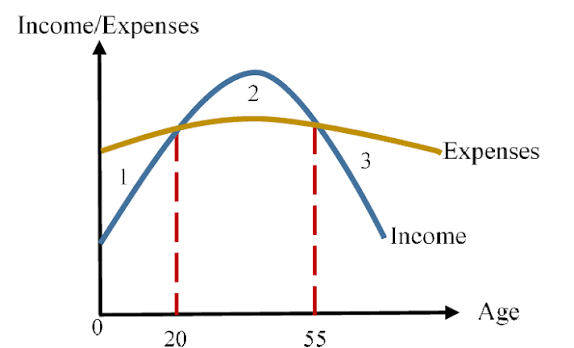
\includegraphics[width=\linewidth]{fig01_life_cycle.png}

            \muted{\scriptsize Life-cycle hypothesis
            \citep{Ando1963_life_cycle, Modigliani1986_life_cycle}, as plotted by
            Rodrigo and Kim (2023).}
        \end{column}
        \begin{column}{0.54\textwidth}
            The hypothesis predicts \bad{decumulation} after retirement;
            housing fits that prediction poorly:
            \begin{itemize}
                \item Illiquidity limits consumption smoothing
                      \citep{Artle1978_life_cycle_homeownership}.
                \item Housing consumption rises early, then \key{plateaus
                      rather than declining} \citep{Yang2009_housing_life_cycle}.
                \item Empirically stable to the end of life
                      \citep{Venti1991_aging_income_value, Venti2004_aging_housing_equity};
                      demand falls mainly at death or on entry into care
                      \citep{Barczyk2023_save_spend_give}.
                \item For most French households the home is the dominant asset
                      \citep{Garbinti2021_wealth_inequality_france} --- a role
                      close to old-age insurance
                      \citep{Power2017_governance_of_ageing}.
            \end{itemize}
        \end{column}
    \end{columns}
\end{frame}

% ============================ 5. THEORY: AGING + SPACE =======================
\begin{frame}{Aging, prices, and space}
    \begin{columns}[T]
        \begin{column}{0.52\textwidth}
            \textbf{The demand channel}
            \begin{itemize}
                \item Flat late-life demand implies aggregate demand
                      \good{holds up} as the population ages
                      \citep{Eichholtz2014_demographics_demand}.
                \item The boomer ``\key{melt-up}'' is documented
                      \citep{Mankiw1989_baby_boom_bust, Takats2012_aging_house_prices}.
                \item The predicted ``meltdown'' appears \bad{not} to be
                      general: it is reported mainly in narrow, high-mortality
                      areas
                      \citep{Dabrowski2019_demography_price_prognosis, Simon2017_concurrence_generationnelle}.
            \end{itemize}
        \end{column}
        \begin{column}{0.48\textwidth}
            \textbf{The spatial channel}
            \begin{itemize}
                \item Aging reshapes territorial dynamics unevenly
                      \citep{EssafiZouari2021_local_housing_wealth}.
                \item And it concentrates population in metropolitan areas
                      \citep{GrafenederWeissteiner2013_agglomeration_demographic, Takahashi2022_aging_economic_geography}.
            \end{itemize}
        \end{column}
    \end{columns}

    \vspace{0.3em}
    \begin{block}{Hypothesis \muted{(following Yang 2009)}}
        If the ``elder boomer'' cohort \key{retains} its housing assets, the
        share of housing wealth held by younger cohorts should grow more slowly.
    \end{block}
\end{frame}

% ============================ 6. TRANSITION ==================================
\transitionslide{Measuring the whole stock}

% ============================ 7. DATA ========================================
\begin{frame}{Two exhaustive administrative databases}
    \begin{columns}[T]
        \begin{column}{0.5\textwidth}
            \textbf{DV3F} --- \muted{transactions (flow)}
            \begin{itemize}
                \item Every recorded French transaction since 2010, with price
                      and detailed property characteristics.
                \item After filtering: \key{430,040} transactions in 2012 and
                      \key{357,820} in 2022.
                \item Drops dwellings under \eur 100 or 9\,m$^2$; IQR outlier
                      removal \emph{by district and year}, so local price
                      dynamics are respected \citep{Kiel2008_location_3L}.
            \end{itemize}
        \end{column}
        \begin{column}{0.5\textwidth}
            \textbf{FF (Fichiers Fonciers)} --- \muted{the stock}
            \begin{itemize}
                \item Every declared residential property, 2012--2022, from tax
                      records.
                \item \key{33.9 million} dwellings in 2012,
                      \key{37.5 million} in 2022.
            \end{itemize}
            \vspace{0.5em}
            Both are processed by CEREMA, carry standardised characteristics and
            precise geolocation, and, importantly for this paper, record the
            \key{owner's age}.
        \end{column}
    \end{columns}

    \vspace{0.4em}
    \muted{\footnotesize All departments except French Guiana and Mayotte.
    Owner age is recorded only for owners born in France.}
\end{frame}

% ============================ 8. MASS APPRAISAL: PROBLEM =====================
\begin{frame}{Imputing prices for the whole stock}
    \begin{columns}[T]
        \begin{column}{0.46\textwidth}
            \begin{block}{The problem}
                The stock file records \emph{who owns what} but carries
                \bad{no prices}. The transaction file carries prices but covers
                only a \bad{small fraction} of the stock each year.
            \end{block}
            \textbf{Mass appraisal:} train on the flow, predict onto the stock
            \citep{Wang2019_mass_appraisal_review}.
            \begin{itemize}
                \item Stratified on \key{14 regional} markets --- homogeneous
                      segments, samples still large enough to train.
                \item Three model types per stratum $\Rightarrow$
                      \key{42 models}.
            \end{itemize}
        \end{column}
        \begin{column}{0.54\textwidth}
            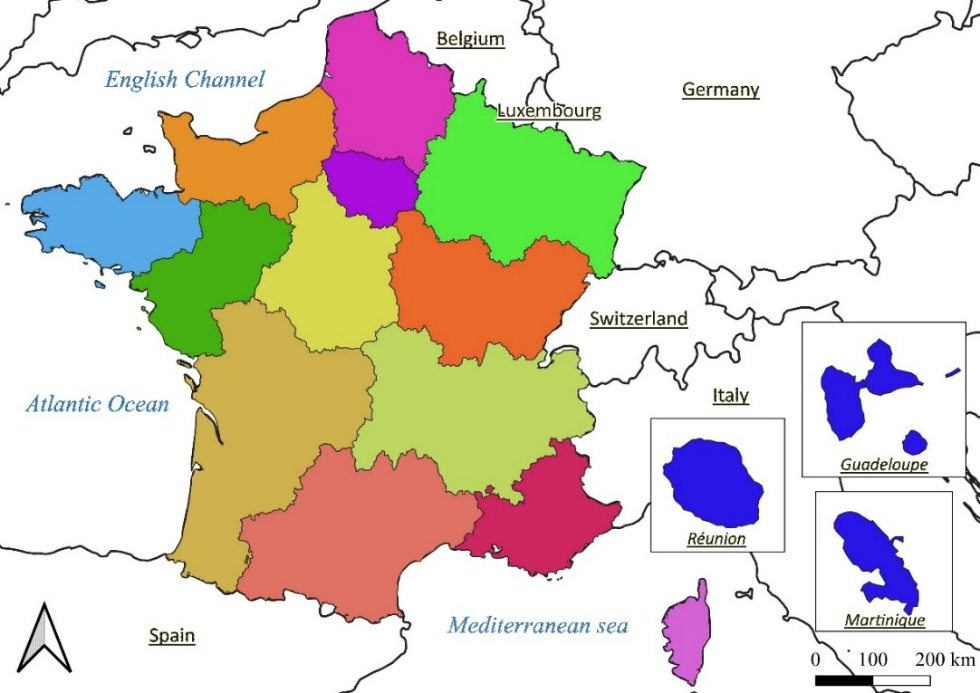
\includegraphics[width=\linewidth]{fig02_strata.jpeg}

            \muted{\scriptsize Figure 2 --- mass-appraisal stratification:
            13 metropolitan regions plus one consolidated overseas model.}
        \end{column}
    \end{columns}
\end{frame}

% ============================ 9. MASS APPRAISAL: CHOICE ======================
\begin{frame}{Model selection and predictive fit}
    \begin{columns}[T]
        \begin{column}{0.54\textwidth}
            \textbf{Three candidates per stratum}
            \begin{itemize}
                \item \textbf{OLS hedonic benchmark} with municipality fixed
                      effects --- grounded in
                      \citet{Lancaster1966_consumer_theory} and
                      \citet{Rosen1974_hedonic_prices}.
                \item \textbf{HGB} and \textbf{XGB} gradient boosting
                      \citep{Chen2016_xgboost_system}, on the same covariates.
            \end{itemize}
            \textbf{Tuning.} 80/20 stratified split; 10,000-iteration random
            grid search; 5-fold cross-validation.
            \begin{itemize}
                \item XGB has the \key{lowest RMSE in 14 of the 15 strata}
                      \muted{(Corse is the exception)}, and is retained.
            \end{itemize}
            \muted{\footnotesize Interpretability is traded away deliberately:
            the target is a \emph{valuation}, not a marginal price
            \citep{Iban2022_explainable_mass_appraisal}.}
        \end{column}
        \begin{column}{0.46\textwidth}
            \centering
            \footnotesize
            \begin{tabular}{lcc}
                \toprule
                \textbf{Mean across strata} & \textbf{RMSE} & \textbf{MAPE} \\
                \midrule
                OLS \muted{(benchmark)} & 0.440 & 4.33 \\
                HGB                     & 0.409 & 3.98 \\
                \textbf{XGB}            & \textbf{0.403} & \textbf{3.94} \\
                \bottomrule
            \end{tabular}

            \vspace{1.0em}
            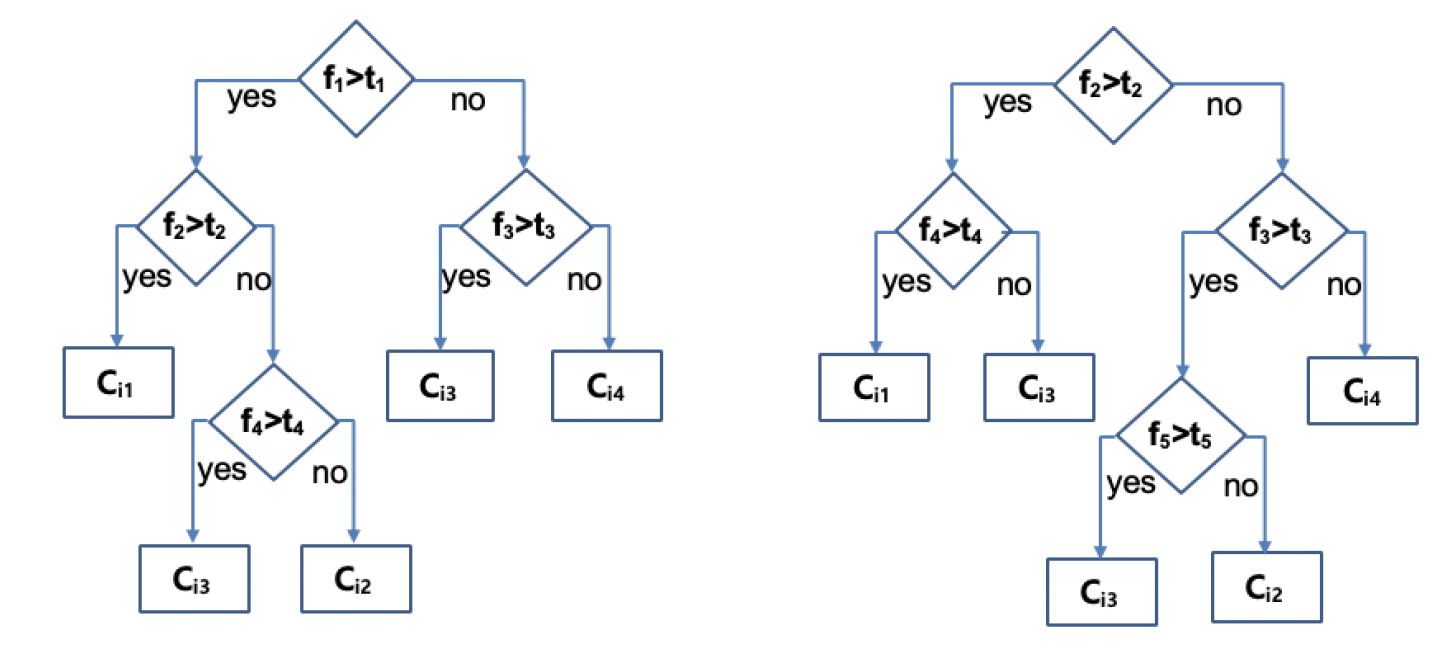
\includegraphics[width=0.94\linewidth]{fig03_decision_tree.png}

            \muted{\scriptsize Figure 3 --- tree partitioning, after
            \citet{Hong2020_random_forest_korea}.}
        \end{column}
    \end{columns}
\end{frame}

% ============================ 10. CONSTRUCTION ===============================
\begin{frame}{From imputed prices to cohort wealth shares}
    Five cohorts --- 18--30, 31--40, 41--50, 51--64, 65+. For each EPCI $i$:

    \begin{equation*}
        K_{a,i} \;=\; \sum_{k \,\in\, (a,i)} P_k ,
        \qquad
        HWE_{a,i} \;=\; \frac{K_{a,i}}{K_i}
    \end{equation*}

    A \emph{cohort} is followed, not an age band --- $\varphi$ maps each 2012 age
    group to where that same cohort sits in 2022:

    \begin{equation*}
        \Delta HWE_{a,i}
        \;=\;
        \frac{HWE^{2022}_{\varphi(a),\,i} - HWE^{2012}_{a,i}}{HWE^{2012}_{a,i}}
    \end{equation*}

    \begin{columns}[T]
        \begin{column}{0.5\textwidth}
            \textbf{Variable of interest.} The log change in the number of
            owners aged \key{65 and over}, 2012--2022.
        \end{column}
        \begin{column}{0.5\textwidth}
            \textbf{Why log differences.} They strip out period-specific levels
            (inflation, credit cost) and time-invariant territorial
            heterogeneity, leaving \key{territorial dynamics}.
        \end{column}
    \end{columns}

    \vspace{0.2em}
    \muted{\footnotesize Controls, all as log changes: physician density,
    employment rate, housing wealth, jobs, secondary residences, birth rate,
    natural increase, net migration.}
\end{frame}

% ============================ 11. SPATIAL ====================================
\begin{frame}{Spatial dependence in the outcome}
    \begin{columns}[T]
        \begin{column}{0.45\textwidth}
            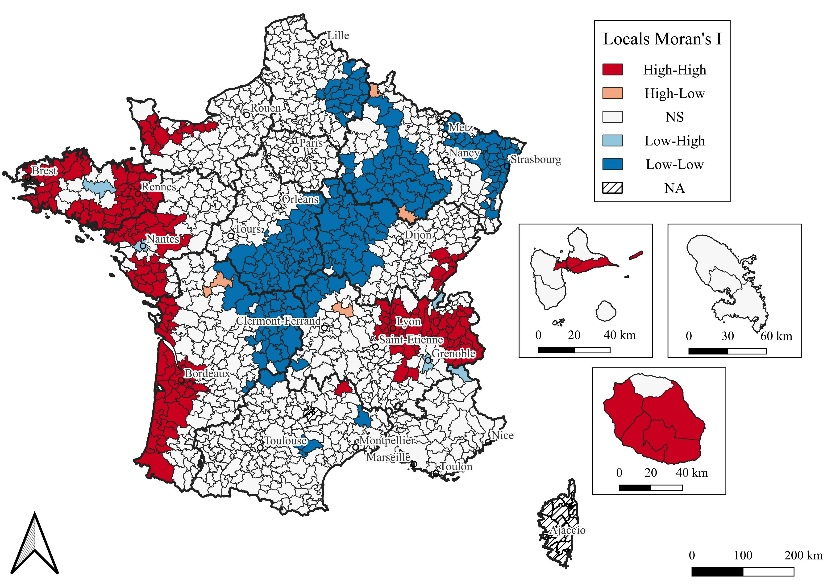
\includegraphics[width=\linewidth]{fig04a_moran_31_40.jpeg}

            \muted{\scriptsize Local Moran's I on $\Delta HWE$ for the 31--40
            cohort in 2022 \citep{Moran1950_continuous_stochastic}.}
        \end{column}
        \begin{column}{0.55\textwidth}
            $\Delta HWE$ is spatially clustered: \textbf{High-High} along the
            Atlantic coast and around Lyon, \textbf{Low-Low} across the rural
            centre and north-east. The clustering \key{widens as cohort age
            rises}.

            \begin{block}{Spatial Durbin Model \muted{(Elhorst 2010)}}
                \vspace{-0.7em}
                \begin{equation*}
                    y = \rho W y + X\beta + W X \theta + \varepsilon
                \end{equation*}
            \end{block}

            \footnotesize
            \begin{itemize}
                \item $W$: \key{Queen contiguity} --- all EPCIs sharing a border.
                \item Lags on \emph{both} the dependent and the explanatory
                      variables \citep{Elhorst2010_raising_the_bar}.
                \item $N =$ \key{1,222} EPCIs. Ignoring spatial dependence
                      would bias OLS; $\rho$ indicates it is present (slide 17).
            \end{itemize}
        \end{column}
    \end{columns}
\end{frame}

% ============================ 12. TRANSITION =================================
\transitionslide{Descriptive evidence: how much, and where}

% ============================ 13. DESCRIPTIVES: AGGREGATE ====================
\begin{frame}{Aggregate growth, and its distribution}
    \begin{columns}[T]
        \begin{column}{0.42\textwidth}
            \begin{block}{Aggregate housing wealth}
                \eur 5.84\,tn \;$\rightarrow$\; \eur 8.05\,tn
                \hfill \key{+38.0\%}

                \vspace{0.3em}
                \muted{2.17$\times$ GDP (2012) $\rightarrow$ 2.9$\times$ GDP (2022)}
            \end{block}

            The aggregate masks substantial heterogeneity. Growth was
            \key{strongest in the upper middle} (p60--p95, all above +25\%) and
            weakest at both tails.

            \vspace{0.3em}
            \muted{\footnotesize In 2022 the top 0.1\% held over \eur 3.12\,m,
            around 33$\times$ the bottom decile's threshold.}
        \end{column}
        \begin{column}{0.58\textwidth}
            \centering
            \footnotesize
            \begin{tabular}{lrrr}
                \toprule
                \textbf{Quantile} & \textbf{2012} & \textbf{2022} & \textbf{Change} \\
                \midrule
                p10                  &    78,855 &    93,481 & +18.6\% \\
                p50 \muted{(median)} &   175,587 &   219,145 & +24.8\% \\
                p90                  &   443,001 &   560,519 & +26.5\% \\
                p99                  & 1,167,872 & 1,434,147 & +22.8\% \\
                p99.9                & 2,661,846 & 3,120,981 & +17.3\% \\
                \bottomrule
            \end{tabular}

            \vspace{0.6em}
            \muted{\scriptsize Housing wealth in euros, per household, owners of
            known age. Selected rows from Table 2.}
        \end{column}
    \end{columns}
\end{frame}

% ============================ 14. DESCRIPTIVES: WEALTH MAP ===================
\begin{frame}{Where housing wealth grew}
    \begin{columns}[T]
        \begin{column}{0.66\textwidth}
            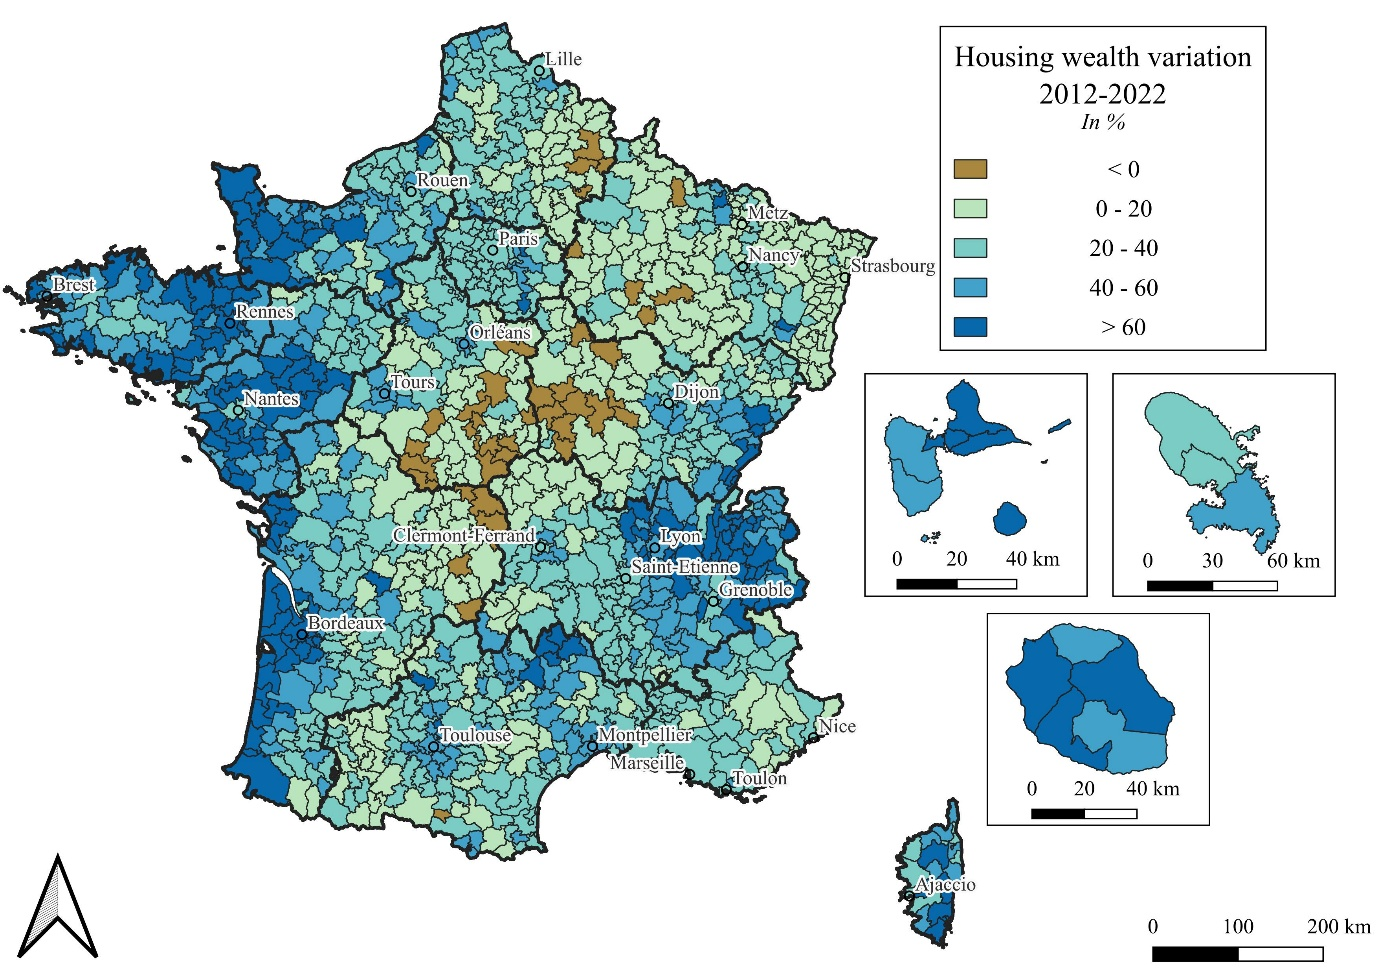
\includegraphics[width=\linewidth]{fig05_wealth_change_epci.jpeg}
        \end{column}
        \begin{column}{0.34\textwidth}
            \footnotesize
            \textbf{Nearly every EPCI gained.}

            \begin{itemize}
                \item \good{Above +60\%}: the coasts, the Swiss and Luxembourg
                      borders, the large metros, Réunion.
                \item \bad{Declines} are few and localised: Nièvre, Yonne,
                      Dordogne, Creuse, parts of the north-east.
                \item These are among the more isolated, rural and rapidly
                      aging territories \citep{Coquard2019_ceux_qui_restent}.
            \end{itemize}
        \end{column}
    \end{columns}
\end{frame}

% ============================ 15. DESCRIPTIVES: AGING MAP ====================
\begin{frame}{Where France aged, 2012--2022}
    \begin{columns}[c]
        \begin{column}{0.37\textwidth}
            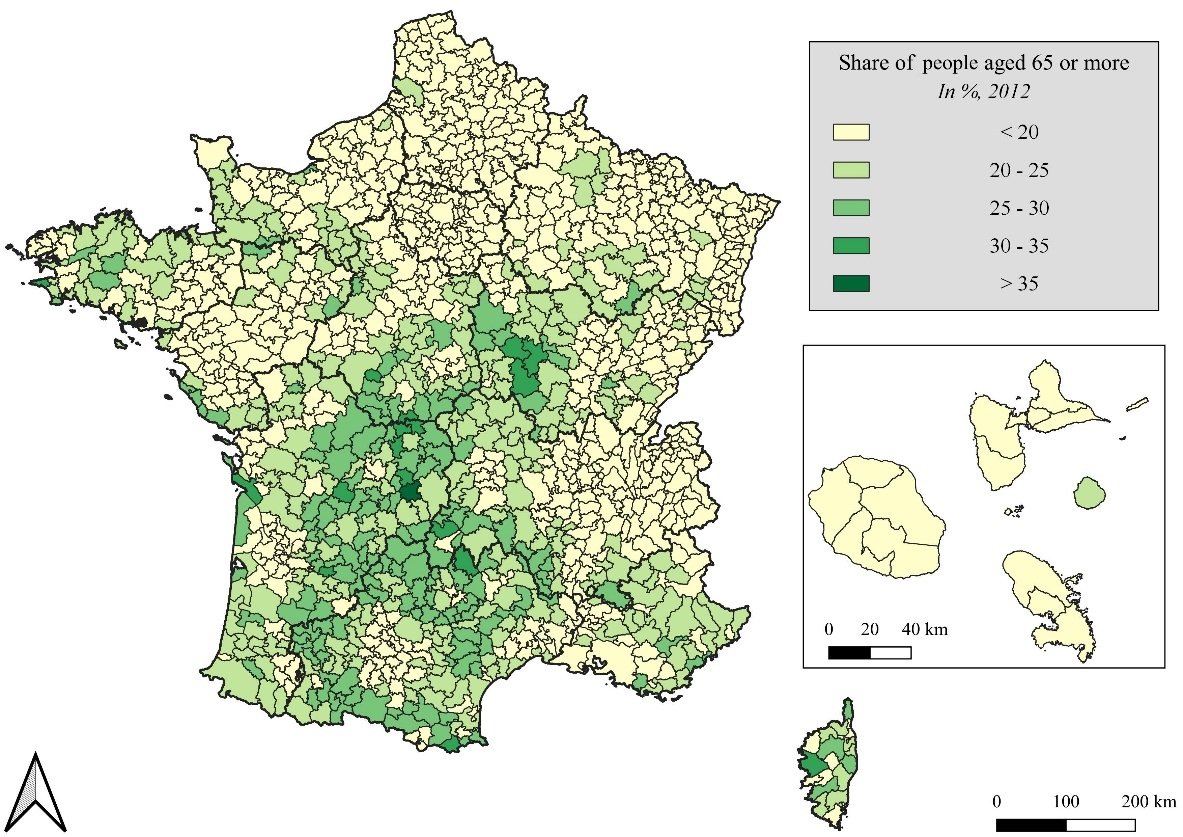
\includegraphics[width=\linewidth]{fig06a_share65_2012.jpeg}
            \begin{center}\muted{\scriptsize 2012}\end{center}
        \end{column}
        \begin{column}{0.37\textwidth}
            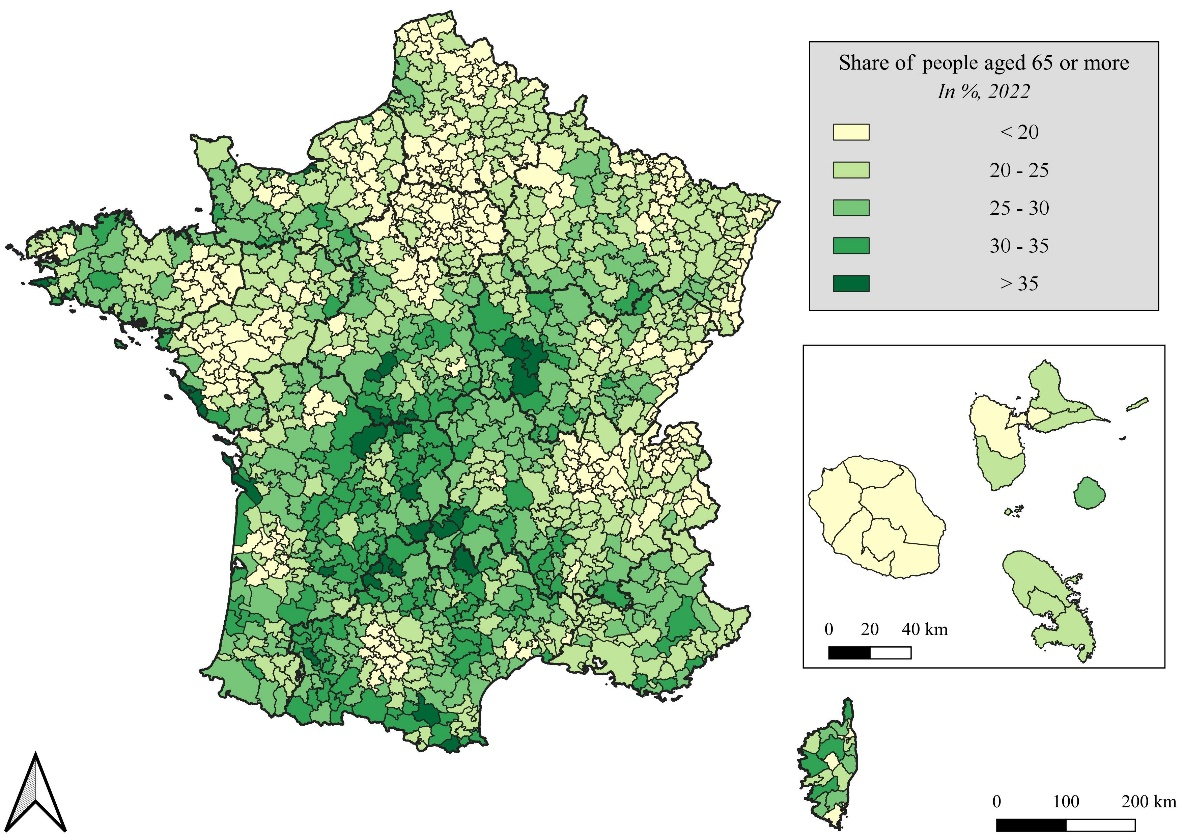
\includegraphics[width=\linewidth]{fig06b_share65_2022.jpeg}
            \begin{center}\muted{\scriptsize 2022}\end{center}
        \end{column}
        \begin{column}{0.26\textwidth}
            \begin{block}{Reading}
                Over the decade, aging \key{intensified existing patterns}
                rather than redistributing the elderly across space.
            \end{block}
            \muted{\footnotesize By 2022 over 35\% of the population is 65+
            across the centre and central-west coast. Île-de-France and Réunion
            stay younger.}

            \vspace{0.2em}
            \muted{\scriptsize Figure 6. Source: INSEE.}
        \end{column}
    \end{columns}
\end{frame}

% ============================ 16. THE CORE FACT ==============================
\begin{frame}{The age distribution of housing wealth, 2012 vs 2022}
    \centering
    % ---------------------------------------------------------------------
    % Figure 7, redrawn. Series are the cached values of the manuscript's
    % embedded Excel chart (word/charts/chart1.xml), verified against the
    % paper's own note (66-75 held 19.42% in 2022, +73.6% over the decade).
    %
    % Geometry: group centres c_i = 0.45 + 1.4i, i = 0..7.
    %   2012 bar spans [c-0.58, c-0.03]; 2022 bar spans [c+0.03, c+0.58].
    %   Vertical scale 0.20 cm per percentage point (tallest bar 24.31 -> 4.86).
    %   y-axis runs to 5.4 cm (= 27 pp); ticks every 5 pp = 1.0 cm.
    %   65+ shading spans x in [6.75, 10.85]; the 56-65 pair ends at 6.63, so
    %   the shading clears it. Legend sits above the plot at y = 5.62..5.87,
    %   clear of the tallest bar (4.86). Region label at (7.05, 4.75) sits
    %   0.87 cm above the 66-75 bar top (3.884) -- Pass 4 boundary rule.
    % resizebox keeps coordinates and text scaling together (Pass P3-safe).
    % ---------------------------------------------------------------------
    \resizebox{0.87\textwidth}{!}{%
    \begin{tikzpicture}[x=1cm, y=1cm]

        % --- 65+ region shading (drawn first, so it sits behind the bars) ---
        \fill[light-bg] (6.75, 0) rectangle (10.85, 5.2);
        \node[primary-blue, font=\footnotesize\bfseries, anchor=west]
            at (7.05, 4.75) {65 and older};

        % --- gridlines, then axes on top ---
        \foreach \pp/\cm in {5/1.0, 10/2.0, 15/3.0, 20/4.0, 25/5.0} {
            \draw[neutral!25, very thin] (-0.25, \cm) -- (11.1, \cm);
        }
        \draw[thick, jet] (-0.25, 0) -- (11.1, 0);
        \draw[thick, jet] (-0.25, 0) -- (-0.25, 5.4);

        % --- y ticks ---
        \foreach \pp/\cm in {0/0, 5/1.0, 10/2.0, 15/3.0, 20/4.0, 25/5.0} {
            \draw[neutral] (-0.38, \cm) -- (-0.25, \cm);
            \node[neutral, font=\scriptsize, left] at (-0.42, \cm) {\pp};
        }
        \node[neutral, font=\scriptsize, rotate=90] at (-1.35, 2.7)
            {Share of national housing wealth (\%)};

        % --- bars: {centre}/{2012 height}/{2022 height}/{age label} ---
        \foreach \c/\ha/\hb/\lab in {
            0.45/0.082/0.080/18--25,
            1.85/1.403/1.400/26--35,
            3.25/3.476/3.130/36--45,
            4.65/4.586/4.203/46--55,
            6.05/4.862/4.470/56--65,
            7.45/3.057/3.884/66--75,
            8.85/1.834/1.976/76--85,
            10.25/0.700/0.857/86+}
        {
            \fill[neutral!45]   (\c-0.58, 0) rectangle (\c-0.03, \ha);
            \fill[primary-blue] (\c+0.03, 0) rectangle (\c+0.58, \hb);
            \node[jet, font=\scriptsize, below] at (\c, -0.14) {\lab};
        }

        % --- legend, above the plot area so it cannot foul the tall bars ---
        \fill[neutral!45]   (3.05, 5.62) rectangle (3.40, 5.87);
        \node[jet, font=\scriptsize, anchor=west] at (3.50, 5.745) {2012};
        \fill[primary-blue] (4.75, 5.62) rectangle (5.10, 5.87);
        \node[jet, font=\scriptsize, anchor=west] at (5.20, 5.745) {2022};

    \end{tikzpicture}}

    \vspace{0.1em}
    {\footnotesize
     \muted{Every cohort under 65 held a smaller share in 2022; every cohort
     65+ held a larger one.}\; 65+ share
     \key{28.0\%\,$\rightarrow$\,33.6\%}; growth \key{+63\%} (65+) vs
     \key{+29\%} (under 65).\par}
\end{frame}

% ============================ 17. SDM ESTIMATES ==============================
\begin{frame}{Spatial Durbin estimates}
    \centering
    \footnotesize
    \begin{tabular}{lccc}
        \toprule
        & \multicolumn{3}{c}{\textbf{Cohort in 2022, dependent variable $\Delta HWE$}} \\
        \cmidrule(lr){2-4}
        & \textbf{31--40} & \textbf{41--50} & \textbf{51--64} \\
        \midrule
        $\Delta$ owners 65+          & $-0.233^{***}$ & $-0.169^{***}$ & $-0.083^{***}$ \\
                                     & (0.019)        & (0.012)        & (0.009)        \\
        \addlinespace
        $\rho$ \muted{(spatial lag)} & $0.514^{***}$  & $0.630^{***}$  & $0.546^{***}$  \\
                                     & (0.033)        & (0.027)        & (0.032)        \\
        \addlinespace
        $N$                          & 1,222 & 1,222 & 1,222 \\
        \bottomrule
    \end{tabular}

    \vspace{0.9em}
    \raggedright
    \begin{columns}[T]
        \begin{column}{0.5\textwidth}
            \begin{itemize}
                \item \key{Negative and significant in all three cohorts}, and
                      larger in magnitude for the younger ones.
                \item $\rho$ is large and highly significant throughout:
                      spatial dependence is \bad{substantial}, which is why the
                      SDM rather than OLS carries the results.
            \end{itemize}
        \end{column}
        \begin{column}{0.5\textwidth}
            \muted{\footnotesize Controls included, not shown. The OLS
            specifications reach $R^2$ of 0.60--0.67. Every SDM coefficient is
            significant except the change in physician density, which matters
            only for the 51--64 cohort. $W$ is a Queen contiguity matrix.
            Selected rows from Table 3.}
        \end{column}
    \end{columns}
\end{frame}

% ============================ 18. EFFECTS ====================================
\begin{frame}{Direct, indirect and total effects}
    \centering
    \footnotesize
    \begin{tabular}{lccc}
        \toprule
        \textbf{Cohort in 2022} & \textbf{Direct} & \textbf{Indirect} & \textbf{Total} \\
                                & \muted{own EPCI} & \muted{neighbours} & \muted{spatial system} \\
        \midrule
        31--40 & $-2.4\%$ & $-1.3\%$ & $\mathbf{-3.7\%}$ \\
        41--50 & $-1.8\%$ & $-1.6\%$ & $\mathbf{-3.4\%}$ \\
        51--64 & $-0.8\%$ & $-0.2\%$ & $\mathbf{-1.0\%}$ \\
        \bottomrule
    \end{tabular}

    \vspace{0.3em}
    \muted{\scriptsize Response of relative housing-wealth growth to a 10\%
    higher growth in the number of owners aged 65+, 2012--2022. Table 4.}

    \vspace{0.6em}
    \raggedright
    \begin{columns}[T]
        \begin{column}{0.5\textwidth}
            \begin{block}{1. A gradient across cohorts}
                The association is stronger for younger cohorts:
                \key{$-3.7\%$} for the 31--40s against $-1.0\%$ for the
                51--64s.
            \end{block}
        \end{column}
        \begin{column}{0.5\textwidth}
            \begin{block}{2. Spatial spillovers}
                Spillovers carry \key{36\%} of the total for the 31--40 cohort
                and 48\% for the 41--50s: retention in one EPCI goes with
                slower growth for younger cohorts in neighbouring EPCIs.
            \end{block}
        \end{column}
    \end{columns}

    \vspace{0.2em}
    \muted{\footnotesize For context, the population aged 18--64 was flat over
    the decade (+0.1\%).}
\end{frame}

% ============================ 19. DISCUSSION =================================
\begin{frame}{Interpretation and limits}
    \footnotesize
    \begin{columns}[T]
        \begin{column}{0.52\textwidth}
            \textbf{The mechanism, and what comes next}
            \begin{itemize}
                \item Consistent with housing-specific life-cycle behaviour
                      \citep{Yang2009_housing_life_cycle}: low mobility and
                      holding to the end, which
                      \citet{Simon2017_concurrence_generationnelle} reads as
                      intergenerational competition for the stock.
                \item Over the next two decades much of this wealth is expected
                      to be transmitted: the \key{``grande transmission''}.
                \item It is likely to land unequally in space --- inheriting in
                      central Paris is not inheriting in the Nièvre
                      \citep{Coquard2019_ceux_qui_restent} --- and asset-based
                      welfare may sharpen that
                      \citep{LeGoix2025_more_volatile_less_equal}.
                \item Dynastic divides may follow, between those who inherit
                      from owners, from renters, or not at all
                      \citep{Cui2024_intergenerational_transfer}.
            \end{itemize}
        \end{column}
        \begin{column}{0.48\textwidth}
            \begin{block}{What we do \bad{not} claim}
                These are \key{robust correlational patterns}, not causal
                estimates.
            \end{block}
            \begin{itemize}
                \item \textbf{Simultaneity.} Retirees may \emph{select into}
                      appreciating markets rather than only cause the change.
                \item \textbf{A composite regressor.} Growth in owners 65+ mixes
                      aging in place, mortality and retiree migration.
                \item \textbf{Imputed values.} The outcome rests on ML
                      predictions --- treat \emph{magnitudes} with care.
                \item \textbf{Interest rates.} The mid-2022 shock falls outside
                      the window.
            \end{itemize}
        \end{column}
    \end{columns}
\end{frame}

% ============================ 20. CONCLUSION =================================
\begin{frame}{Conclusion}
    \begin{block}{The finding}
        Between 2012 and 2022, the aging of the boomer cohort is associated with
        \key{lower housing-wealth growth for the younger cohorts in France}, an
        association that is stronger for the youngest and that extends across
        space into neighbouring territories.
    \end{block}

    \begin{itemize}
        \item The pattern is consistent with population aging operating as a
              \key{structural constraint} on housing-wealth accumulation, rather
              than as a purely compositional shift.
        \item Demographic decline may eventually rebalance the distribution, but
              on a horizon of several decades; the gap is unlikely to close in
              the interim.
        \item This suggests demography belongs alongside class in housing-policy
              analysis: the cohort is large enough for its size to matter on its
              own.
    \end{itemize}

    \vspace{0.2em}
    \textbf{Two policy directions currently discussed.} Reforming inheritance
    taxation \citep{Dherbecourt2021_repenser_heritage}, or developing
    equity-release and \emph{viager} instruments
    \citep{Coulomb2021_viager_territoires, Coulomb2025_epargne_capturee}.
    \muted{Plausibly complementary, given the scale of the transfer to come.}
\end{frame}

% ==================== REFERENCES (unnumbered, not one of the 20) =============
\begin{frame}[noframenumbering, allowframebreaks]{References}
    \tiny
    \bibliography{../Bibliography_base}
\end{frame}

\end{document}
